\chapter{Background and Related Work}\label{C:back}

\section{General Networking}

Information which is sent across a network is generally divided into smaller pieces. When each piece
traverses a network, extra information is repeatedly added and removed until it has arrived at the
destination. This extra information is split into multiple layers and each layer has a different function.
The Open Systems Interconnection (OSI) model (Figure: \ref{fig:OSIModel}) is a widely implemented standard that
defines these different layers of extra information and their purpose.

\begin{figure}[H]
    \begin{center}
        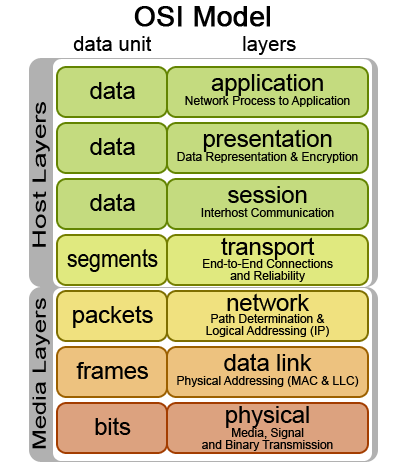
\includegraphics[width=5cm,height=5cm,keepaspectratio]{Images/OSIModel.png}
        \caption{OSI Model \cite{OSIPic}}
        \label{fig:OSIModel}
    \end{center}
\end{figure}

Network switches and network routers interpret the destination based off information found in
Layer 2 or Layer 3 from the OSI model, hence I must adhere to the protocol standards found at these
layers. Layers 4 and above provide other benefits to the payload such as reliability and is not a
concern for this project.

\subsection{Layer 1}

In Ethernet systems, Layer 1 refers to the physical medium that information is being sent over.
Gigabit ethernet based systems use a copper wire as the physical medium, with electrical voltages
representing the information. For this project, the latency is measured at this layer.

\subsection{Layer 2}

Layer 2 is responsible for transferring data between adjacent network devices \cite{IEEE802}. This is important as
information will be flowing to and from adjacent nodes, through a switch or router. To ensure that
information flows through the switch or router, this layer must be taken into consideration to ensure
successful transmission and reception of information.
This layer is important to the project as the measuring device will be timing the latency between adjacent 
network devices and through network switches, both of which rely on Layer 2 information.

\subsection{Layer 3}

Information from one hop to another is determined by the Layer 3 protocol. This ensures that
information is correctly routed to the destination from the source. This layer is important as the
information stored at this layer ensures the correct path is taken from sender to receiver. This is
different to Layer 2, as this can incorporate non-adjacent nodes as well.

\section{Latency Definitions}

For this project, latency in a network will be defined in the following ways. 
This project will be focusing on One Way Trip time, because it is a subset of the other latencies.

\subsection{Connection Time}

Connection time describes the time that two devices take to enable information flow between them. In
some cases, there are many synchronisation and authentication steps that need to take place before
any information can flow. This latency is defined as the initialization of the first command, to the
processing of the final command.

\subsection{Return Trip Time}

In some cases, the return trip time can be used to measure the one-way latency of two devices. One
device sends a request for an echo and when the echo is recieved, the time taken from transmition to reception is
twice the latency between devices.

\subsection{One way Trip Time}

This is similar to Return Trip Time but instead of requiring an echo back to the sender, the receiver is on the
same device. Hence the latency of the connection is measured as the time taken for the information
to flow from one port on the device to another.

\section{Current Solutions}

There are solutions present which can measure latency to a high degree (< 1 ms) but have some drawbacks in different areas.
These can be split into two different catagories, hardware and software, referring to the process of which they measure latency.

\subsection{Software}

\subsubsection{Ping}

Ping is a Linux utility that can be used to estimate the latency to a given network server. 
This is for large distance measurements, as the accuracy of this ranges from seconds to milliseconds. 
It has also been tested that this utility is unreliable for performance extensive testing as momentary ‘glitches’ 
can appear in networks, causing random and unpredictable results \cite{pingisbad}.
It is very useful at measuring very large latencies (>1 milliseconds) and displaying them in a concise format 
for analysis by the user. 
This does not meet the need of having the ability to measure time in the nanosecond range, but a useful takeaway 
is to make sure that values are presented in an easy to analyse format (printing to screen, or to a file).

\subsubsection{Data plane Development Kit (DPDK)}

DPDK is a software implementation of rapid packet processing. 
This software utilises low level software drivers to interact directly with the hardware. 
Doing so requires specific hardware on the computer which needs to be compatible with the software itself.
Reducing the packet processing time reduces the time offset created by the CPU, but not fully removes it. 
Examples in the source code have shown that the timing value is dependent on CPU frequencies \cite{dpdkcode} 
and Dynamic Frequency scaling \cite{turboboost} of modern CPUs can cause a change in this frequency at any time.
An advantage of this solution is that it can produce a high-resolution time value (in the order of nanoseconds) 
and is easily accessible by a user in software for processing and analysing. 
A lesson learnt from this approach is that a CPU based system for measuring high resolution timers will not be precise or accurate.

\subsubsection{PF\textunderscore RING}

Another software solution is PF\textunderscore RING by ntop\texttrademark. 
It is a rapid packet processing library that does not require the need for specific hardware.  
PF\textunderscore RING allows for more efficient packet capturing and filtering by utilising more cores and threads on a CPU \cite{pfringworks}.
This library is more focused on throughput of packets processed rather than latency. 
This is less accurate than the DPDK but increases the flexibility of the platform it can implemented on. 
As with all software based approaches, this does not meet the requirements of being able to measure time in nanoseconds reliably.
An insight from this approach is to flexibility of platform is good for users but will not be a requirement for this project.

\subsection{Hardware}

\subsubsection{Data Acquisition and Generation (DAG) 10x2-S}

\par The DAG 10x2-S by Endace is a hardware based packet capturing solution with high precision nanosecond scale precision \cite{dagprecision}. 
This is a physical device which connects to a x86 based computer and communicates via Peripheral Component Interconnect Express (PCIe). 
The DAG 10x2-S is recommended for capturing network packets over gigabit ethernet links, as the other models cost more and have other unnecessary features \cite{dagfeatures}.
It is an expansion card for a computer which extends the capabilities of the computer to accurately capture and timestamp packets to a high degree. 
This device has the capabilities to timestamp packets with a resolution of 4ns \cite{dagprecision}. 
This meets all the requirements of the project but is very costly (\$2500 USD \cite{dagprice}) and methods for obtaining a device can only be done through Endace themselves. 

\subsubsection{Field Programmable Gate Array (FPGA)}

\par A FPGA is an array of configurable logic gates. The number of gates are in the order of thousands to
millions. This many configurable gates allows for complex logical structures and digital circuits to be
implemented in hardware, while consuming little physical space. This differs from a CPU, where the
logical gate circuitry is fixed, and manipulation of electrical Input/output must be done by clocking
through an instruction set. Without the need for an instruction set, FPGAs allow for high speed time
critical applications to be implemented without the overhead of needing to clock through CPU
instructions. This is an important characteristic as the electrical signals measured from the network
interfaces are time critical.

\subsubsection{NetFPGA-SUME Virtex-7 FPGA Development Board}

\par The NetFPGA-SUME is a FPGA development board for high density and high-performance networking design.
This incorporates a FPGA to process packets rapidly in hardware, much faster than any software.
The Virtex-7 FPGA onboard is a recently released FPGA which can process up to 13.1 gigabits per second worth 
of information through its transceivers while the scope of this project is limited to 1 gigabit per second 
ethernet.
This is also a very costly development board, costing \$4999 \cite{SUME} for academic customers. 
Due to the limited scope of this project and the cost involved with purchasing this development board, this is 
not a suitable platform for developing latency measuring device.

\subsubsection{Xilinx Zynq FPGA}

\par Xilinx is a manufacturer of FPGAs, and a family of products they produce is the Zynq-7000 range \cite{fpga}.
These FPGAs integrate a dual-core ARM Cortex-A9 MPCore with FPGA gate fabric enabling high performance 
applications to run on the FPGA, while embedded programs can run on the ARM cores.
This project incorporates the FPGA section to manage the timing functions and the ARM section to run the 
application for storing the timing information.

\section{Related Work}

\subsection{Moongen}

\par MoonGen is a flexible high-speed network packet generator. The goal was to saturate 10 Gb Ethernet links using 
a flexible hardware platform. A key issue defined in the paper was that Existing software solutions lack performance
or flexibility when precision is desired. Existing hardware solutions are expensive with inflexible software accompanying
the platform. A key takeaway is that existing platforms are inflexible and lack precision.

\subsection{Flexible High Performance Traffic Generation on Commodity Multi–Core Platforms}

\par A similar problem is solved with this paper. The goal was to saturate a 10 Gb Ethernet link using software methods.
Another mention of inflexible hardware solutions was present in this paper, alluding to the fact that existing
solutions that are based on hardware are lacking in flexiblity. This may seem to say that a hardware based solution may
not be the correct approach to measuring latency, but this shows the novelty in a solution that is flexible
and hardware based.

\subsection{A Distributed Instrument for Performance Analysis of Real-Time Ethernet Networks}

\section{Hardware Implementation}

\subsection{Differential Signaling}

\par Differential Signalling is a method of electrical communication using opposing electrical voltages on two wires. 
This is advantageous in transmission of electrical signals in electrically noisy environments as no reference 
point is used to infer information. If a reference point is used in an electrically noisy environment, the 
noise can couple to the reference point, causing errors in the information transferred. Differential signalling 
removes this dependency on a reference point by transferring information through the difference between the two 
transmission lines. By twisting the transmission lines together, external electrical signals are coupled to both 
lines, and do not affect the difference between the two lines. This way information is transferred over a large 
distance reliably and at high speed. In Gigabit Ethernet, information is transferred through 4 pairs of twisted 
differential paired cables.

\subsection{Pulse Amplitude Modulation}

\par Pulse Amplitude modulation is a form of modulating a signal with information encoded in discrete levels of pulses.
Different versions of PAM have varying levels of discrete steps. In Gigabit Ethernet, PAM-5 is used with 5 
different voltage levels each corresponding to different set of predefined binary codes interpreted by the 
decoder.

\subsection{IEEE 802.3ab}

\par IEEE 802.3ab is the defining standard for gigabit ethernet communication across a copper link. 
It defines the use of 4 pairs of copper and the maximum length (100 m) the protocol is designed for.
Ethernet Physical Transceiver (Ethernet PHY)
An Ethernet PHY is an electronic component used to convert signalling from a link layer device (Such as a MAC) 
to the physical layer (differential signalling with PAM). Common interfaces to communicate from a MAC to a PHY 
include GMII, RGMII, XGMII.

\subsection{Gigabit Media Independent Interface (GMII)}

(GMII IMAGE HERE)

\par GMII is a protocol used in this project to communicate between the Ethernet PHY and the MAC which is implemented 
on the FPGA. The ethernet PHY decodes the data sent from the GMII interface, and produces the correct signalling 
required for the receiving Etherenet PHY. The process of clocking out data requires 8 data line connections, 
and a few extra lines for timing/scheduling.

\subsection{Reduced GMII (RGMII)}

(RGMII Signals HERE)

\par RGMII is an implemenetation of GMII, but a key difference is a reduction in the number of transmit lines. This is
possible through the use of clocking all signals on a bus consisting of Dual-Data-Rate (DDR) lines. This is done through 
clocking the data in and out on both the rsising edge and the falling edge of the clock. This helps reduce the number
of physical wires used to interconnect components on the PCB, making more space for routing other complex busses (Such as
DDR3 for the RAM).

\subsection{Advanced Microcontroller Bus Architecture}

\subsection{Advanced eXtensible Interface}

\subsection{Serial Peripheral Interface}
